\documentclass[UTF8]{ctexart}
\usepackage{algpseudocode}
\usepackage{algorithm}
\usepackage{amsmath}
\usepackage{subcaption}
\usepackage{graphicx}
\usepackage[top=4em,bottom=4em]{geometry}
\usepackage{lmodern}
\usepackage{listings}
\usepackage{xcolor}

\ctexset{ section = { format={\Large \bfseries } } }

\pagestyle{empty}

\begin{document}

\section*{Task 1: Inverse Kinematics}

\subsection*{Sub-Task 1, 2, 3}

直接按照算法流程实现。

\begin{figure}[htbp]
    \hfill
    \begin{subfigure}[b]{0.49\textwidth}
        \centering
        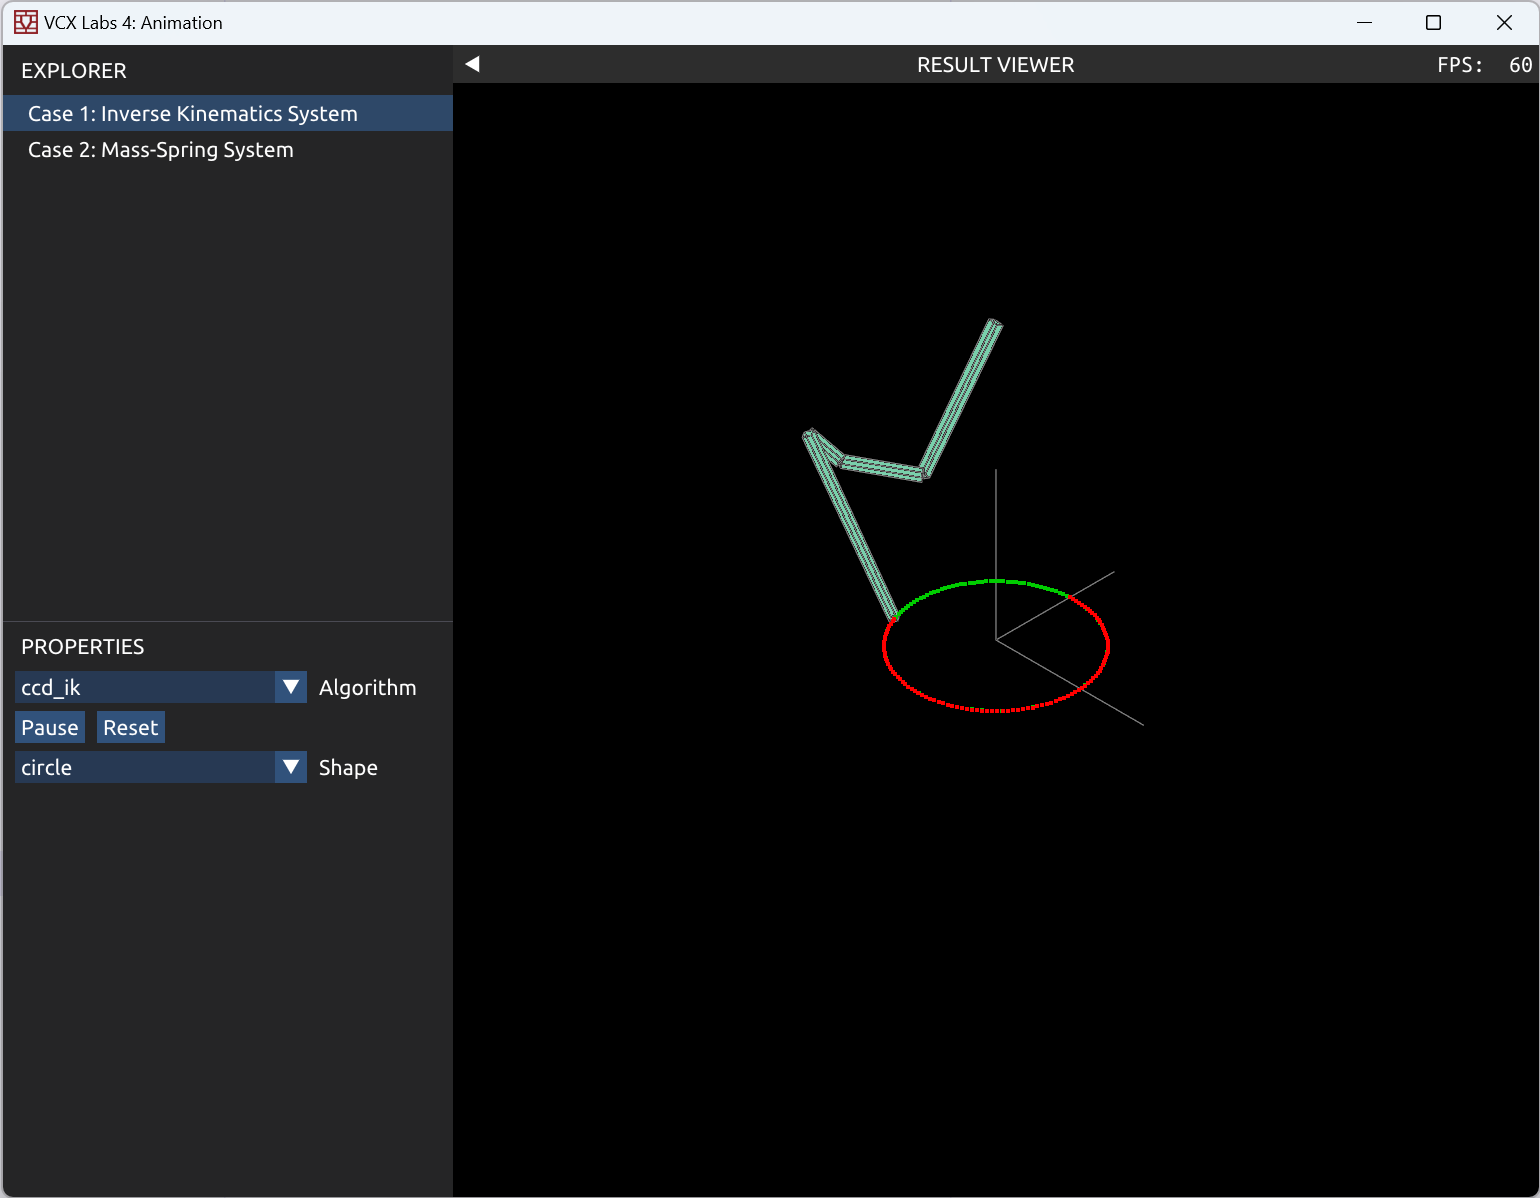
\includegraphics[width=\textwidth]{images/1-1.png}
        \caption{CCD IK}
    \end{subfigure}
    \hfill
    \begin{subfigure}[b]{0.49\textwidth}
        \centering
        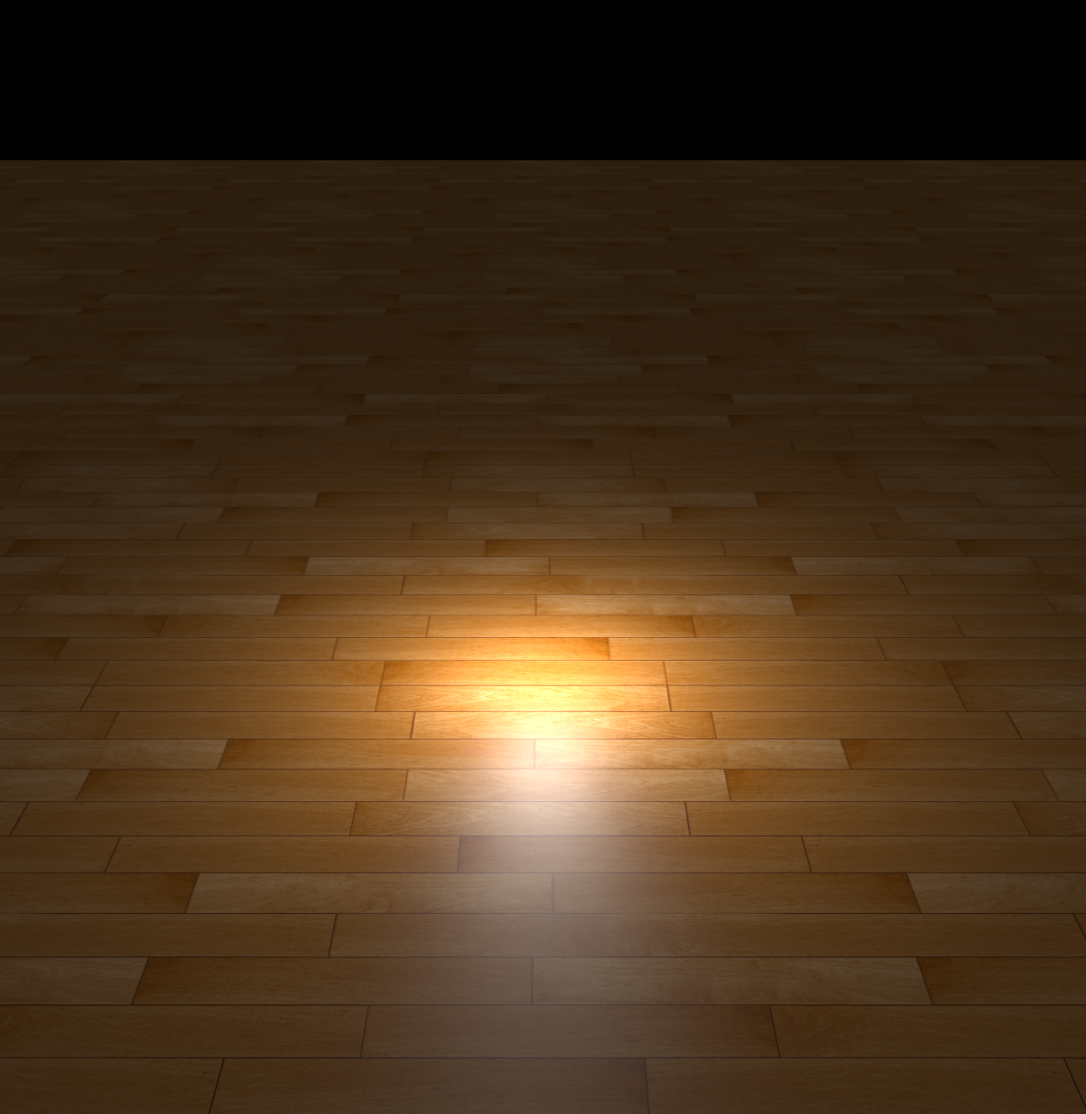
\includegraphics[width=\textwidth]{images/1-2.png}
        \caption{FABR IK}
    \end{subfigure}
    \hfill
    \caption*{Task 1}
\end{figure}

\subsection*{Sub-Task 4}

自定义了一些数字。

\begin{figure}[htbp]
    \centering
    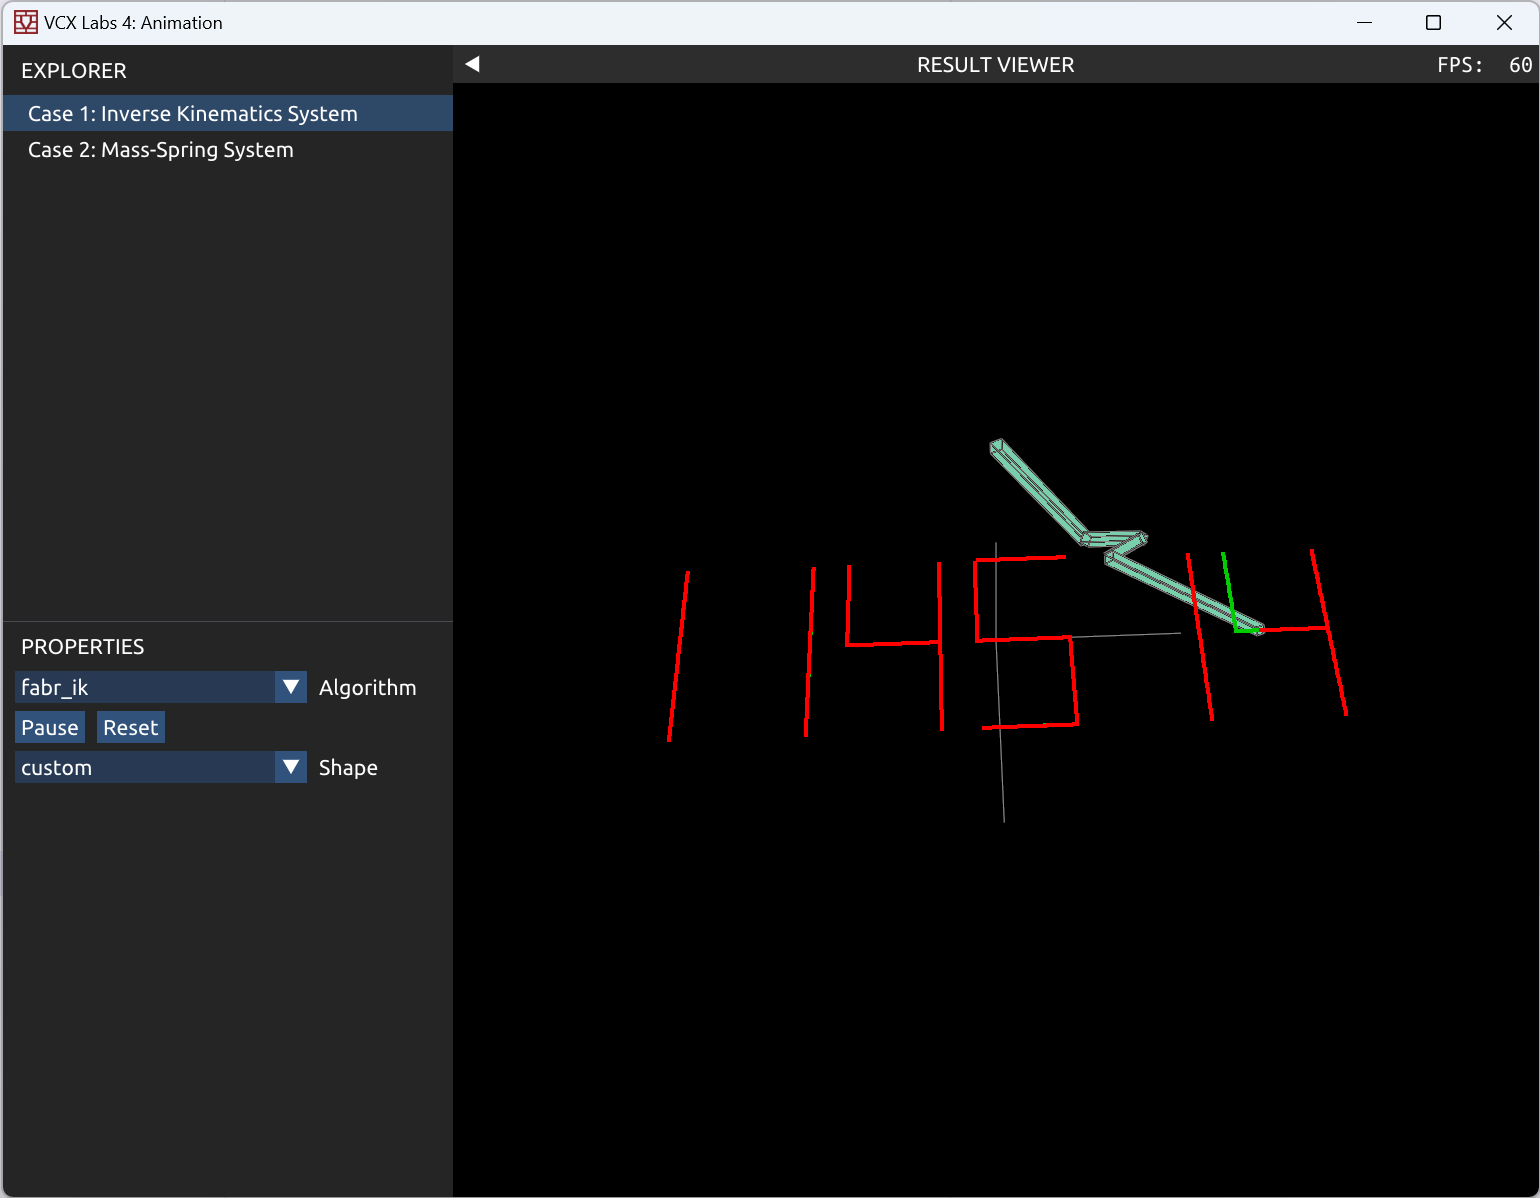
\includegraphics[width=0.8\textwidth]{images/1-3.png}
    \caption*{Sub-Task 4}
\end{figure}

\subsection*{问题}

\begin{enumerate}
    \item {\kaishu 如果目标位置太远,无法到达,IK 结果会怎样?}
    \begin{itemize}
        \item 在一定迭代次数后,机械臂会收敛到朝向目标位置伸直的状态。
    \end{itemize}
    \item {\kaishu 比较 CCD IK 和 FABR IK 所需要的迭代次数。}
    \begin{itemize}
        \item CCD IK 需要的迭代次数较多,在这个 Lab 的任务中大多数情况都到达了上限 100,这意味着要达到目标精度实际上仍需要更多次迭代。
        \item FABR IK 迭代次数较少,在这个 Lab 的任务中大多数情况迭代次数不超过 4,不过若目标距离比较接近机械臂的最大长度时可能会出现 30 到 50 的迭代次数。
    \end{itemize}
\end{enumerate}

\section*{Task 2: Mass-Spring System}

设当前时间点所有质点的位置和速度分别为 $x_n, v_n$。则时间 $h$ 后的位置和速度分别为
\begin{align*}
    x_{n+1} &= x_n + \Delta x = x_n + h v_{n+1}, \\
    v_{n+1} &= v_n + \Delta v = v_n + h \left(g + \frac{f(x_{n+1}, v_{n+1})}{m}\right),
\end{align*}
其中 $g$ 为重力加速度,$m$ 为质量,$f$ 为受力函数。为了简化计算,使用泰勒级数展开,得到一阶近似
\begin{align*}
    f(x_{n+1}, v_{n+1}) = f(x_n, v_n) + \frac{\partial f}{\partial x} \Delta x + \frac{\partial f}{\partial v} \Delta v.
\end{align*}
将要求解的 $v_{n+1}$ 移到左边,得到
\begin{align*}
    \left(1 - \frac{h^2}{m} \cdot \frac{\partial f}{\partial x} - \frac{h}{m} \cdot \frac{\partial f}{\partial v}\right) v_{n+1} = v_n + h \left(g + \frac{1}{m}\left(f(x_n, v_n) + \frac{\partial f}{\partial v} \cdot v_n\right)\right).
\end{align*}
为了简化计算,认为 $\partial f / \partial v = 0$,也即忽略了 damping 的隐式求解。由于隐式方法耗时较长,减小迭代次数至 $10$,效果如下。

\begin{figure}[htbp]
    \centering
    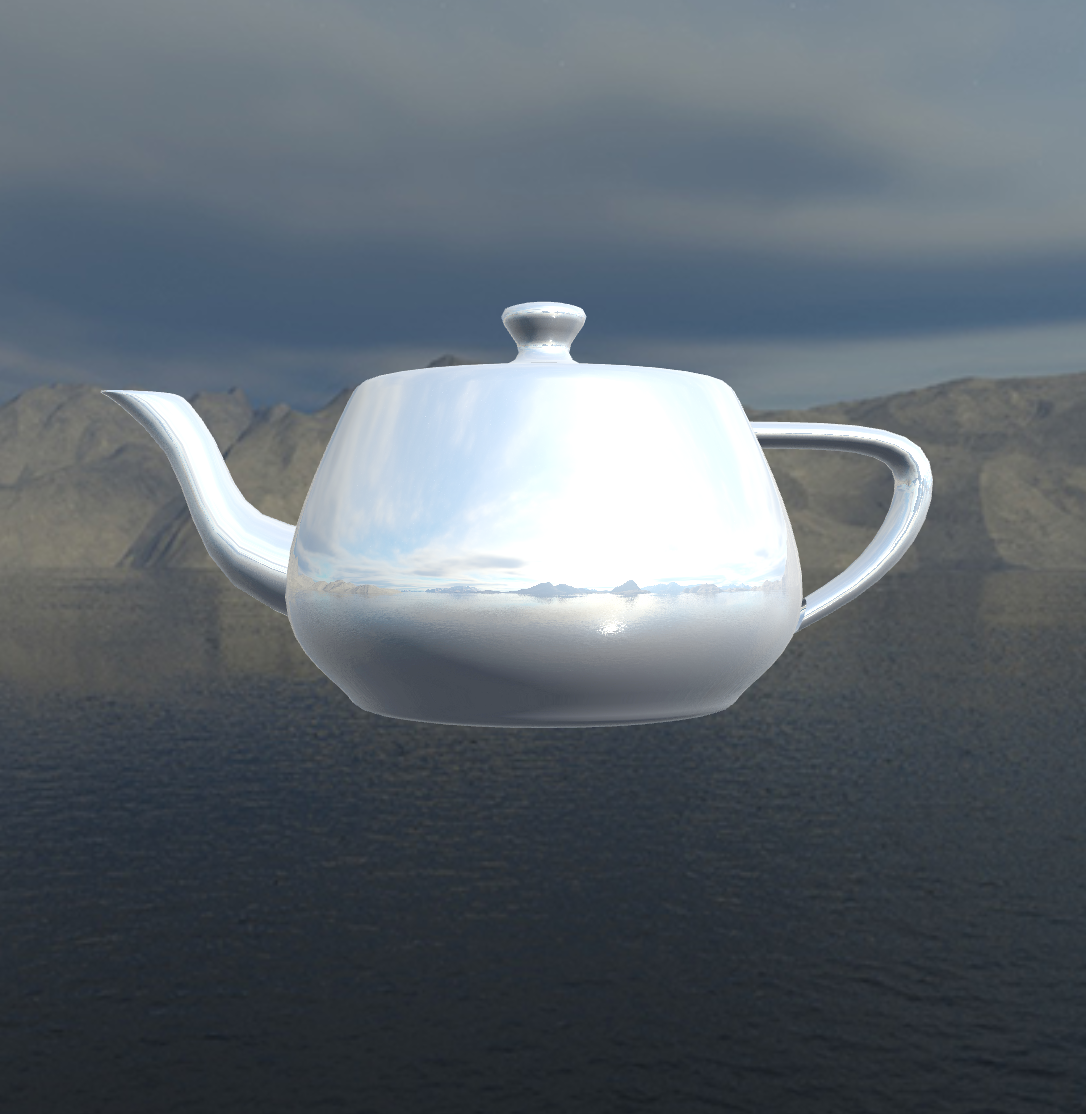
\includegraphics[width=0.9\textwidth]{images/2-1.png}
    \caption*{Task 2}
\end{figure}

\end{document}